% Формат дипломной работы:
%     - шрифт 14
%     - бумага А4
%     - поля 2х2х2х2см
%     - полуторный межстрочный интервал
\documentclass[14pt]{extarticle}
\usepackage[paper=a4paper, top=2cm, bottom=2cm, right=1cm, left=3cm]{geometry}
\linespread{1.25}

% Стиль оглавления
%\usepackage{titletoc}
%\titlecontents{section}[2em]{\bfseries\addvspace{0.5em}}
%{\contentslabel[\thecontentslabel]{1.7em}}
%{}{\titlerule*[1pc]{.}\contentspage}
% Необходимые пакеты для компиляции русского языка, картинок и прочего

\usepackage[utf8]{inputenc}                % Кодировка
\usepackage[main=russian, english]{babel}  % Русский язык
\usepackage[pdftex]{graphicx}              % Картинки
\usepackage{indentfirst}                   % Отступ перед абзацами

\usepackage{amsmath}  % Математические 
\usepackage{amssymb}  % формулы
\usepackage{scalerel}

\usepackage{tikz}  % Векторная графика

\usepackage{xcolor} % Цветной текст для заметок

\usepackage[unicode]{hyperref}                           % Ссылки и русские закладки
\hypersetup {                                            %
    pdftitle={Выпускная квалификационная работа},        % Название документа
    pdfsubject={Математическое моделирование движений руки, держащей предмет}, % Тема документа
    pdfauthor={Егоров Кирилл Юлианович},                 % Автор документа
    pdfcreator={Кафедра системного анализа ВМК МГУ},     % Создатель документа
    pdfproducer={LaTeX},                                 % Программа, создавшая документ
    hidelinks                                            % Скрывает рамку вокруг ссылок
}

\usepackage{amsthm}  % Красивый внешний вид теорем, определений и доказательств
\newtheoremstyle{def}
        {\topsep}
        {\topsep}
        {\normalfont}
        {\parindent}
        {\bfseries}
        {.}
        {.5em}
        {}
\theoremstyle{def}
\newtheorem{definition}{Определение}
\newtheorem{example}{Пример}

\newtheoremstyle{th}
        {\topsep}
        {\topsep}
        {\itshape}
        {\parindent}
        {\bfseries}
        {.}
        {.5em}
        {}
\theoremstyle{th}
\newtheorem{theorem}{Теорема}
\newtheorem{lemma}{Лемма}
\newtheorem{assertion}{Утверждение}

\newtheoremstyle{rem}
        {0.5\topsep}
        {0.5\topsep}
        {\normalfont}
        {\parindent}
        {\itshape}
        {.}
        {.5em}
        {}
\theoremstyle{rem}
\newtheorem{remark}{Замечание}

% Новое доказательство
\renewenvironment{proof}{\parД о к а з а т е л ь с т в о.}{\hfill$\blacksquare$}
\newcommand{\T}{^\mathrm{T}}

\usepackage{subfiles}
\graphicspath{{\subfix{./img}}}
\begin{document}
        \thispagestyle{empty}
\begin{center}
    \ \vspace{-3cm}

    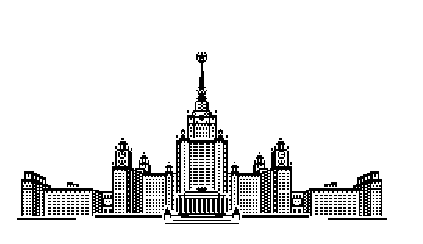
\includegraphics[width=0.5\textwidth]{title_page/msu.eps}\\

    {\small{\scshape  Московский государственный университет имени М.~В.~Ломоносова}\\
    Факультет вычислительной математики и кибернетики\\
    Кафедра системного анализа}

    \vfill

    {\Large Егоров Кирилл Юлианович}

    \vspace{1cm}

    {\LARGE\bfseries Математическое моделирование движений руки,
    держащей предмет}

    \vspace{1.5cm}

    {\scshape магистерская диссертация}
\end{center}

\vspace{3cm}

\begin{flushright}
    \large
    \textit{Научный руководитель}\\
    к.ф.-м.н., доцент И.\,В.~Востриков
\end{flushright}

\vfill

\begin{center}
    Москва, 2023
\end{center}

\clearpage
        \tableofcontents
        \clearpage
        %\clearpage
        %\documentclass[../doc.tex]{subfiles}
\graphicspath{{\subfix{../img}}}
\begin{document}
    Работа посвящена построению оптимальных траекторий движения в модели бионической руки человека,
        держащего предмет.
    Целью работы является построение эффективного вычислительного метода
        для управления сложными биомеханическими системами.
    Для разработки и тестирования построенного метода
        была предложена соответствующая математическая модель.
    
    Исследования в области биологического движения имеют огромное практическое значение:
        они позволяют частично восстановить двигательную фун\-кцию у людей
        с ограниченными возможностями,
        чем существенно улучшить качество их жизни.
    Последние технические достижения в области роботизированных протезов
        и функциональной электронной стимуляции парализованных мышц
        позволяют начать внедрение данной теории.
    Более того, сложные бионические устройства становятся бесполезными без соответствующего знания
        о грамотном управлении ими.
    
    Актуальность данной сферы исследований подтверждается наличием большого числа работ последнего времени,
        улучшающих существующие методы решения задач, связанных с биологическим движением, таких как \cite{maneeshika2023}, \cite{wang2008},
        а также работ,
        предлагающих новые математические модели для отдельных аспектов движения, например, \cite{maroger2022}.

    В работе предложена математическая модель руки человека, держащего предмет,
        как планарного трёхсекционного математического маятника.
    Выведена динамика данной физической системы.
    Для возможности анализа поведения системы методами оптимального управления
        постулирован принцип оптимальности
        и рассмотрены представленные в литературе (\cite{hogan1984}, \cite{uno1989}) формализации
        оптимизационного энергетического критерия.
    
    Использование методов оптимального управления способно привести фундаментальным открытиям в области
        биологической моторики: от описания свойств функций отдельных мышц, до исследования контроля
        мышц нервной системой при выполнении целевых задач, ---
        поскольку данные методы напрямую работают с причинами движений, выраженными в форме оптимизационных критериев.

    По результатам математического моделирования была поставлена задача оптимального целевого управления нелинейной системой в непрерывной и дискретной формах.
    В качестве управления выбрано изменение крутящего момента каждого из сочленений.
    В работе полагается отсутствие ограничений на управление и известное полное фазовое состояние системы.

    Для решения задачи в дискретной постановке были рассмотрены известные базовые методы решения задачи
        оптимального управления нелинейными системами~\cite{murray1984}, \cite{li2004}.
    В качестве основного метода в данной работе применяется итеративный метод,
        предполагающий последовательное построение серии линейно-квадратичных регуляторов
        для системы и функционала качества, аппроксимированных вдоль заданной траектории.
    
    При разработке метода особое внимание было уделено аспектам, не достаточно подробно
        изложенным в литературе: способу регуляризации оптимальной поправки и способу
        построения начальной референсной траектории без опоры на мнение эксперта в предметной
        области.

    Полученное в результате программное решение, реализующее предложенный метод, 
        было применено для рассмотрения конкретных постановок задачи~---
        классических задач биомеханического движения: задача целевого положения схвата, задача обхода препятствия.
    Они служат возможности сравнения результатов работы предложенного метода с имеющимися в литературе, например, с \cite{mitrovic2010}, \cite{todorov2005}.

    Результаты, полученные в рамках работы над диссертацией, были представлены в качестве доклада на научной конференции
    <<Ломоносовские чтения -- 2023>> \cite{egorov2023}.

    \ifSubfilesClassLoaded{
        \nocite{*}
        \clearpage
        \bibliographystyle{plain}
        \bibliography{../../refs}
    }{}
\end{document}
        %\clearpage
        %\section{Математическое моделирование}

\subsection{Дискретизация задачи}

{\color{red} Тут уже чувствуется, что буквы начали повторяться.}

Для удобства дальнейших рассуждений дискретизируем задачу~\eqref{eq:kinematic}-\eqref{eq:cauchy}-\eqref{eq:continuos-cost} по времени $t_0 \leqslant t \leqslant t_1$.
Для этого введем равномерную сетку с шагом~$\Delta t$:
$$
    \{ t_i \}_{i=0}^{N+1}, \quad t_0 = t_0, \quad t_N = t_1, \quad t_{i+1} - t_{i} = \Delta t.
$$
Тогда, сузив класс допустимых управлений до кусочно-постоянных, получаем дискретный вариант рассматриваемой задачи Коши~\eqref{eq:kinematic}-\eqref{eq:cauchy}:
\begin{equation}\label{eq:discrete-system}
    \left\{\begin{aligned}
        &x^{k+1} = f(x^k, u^k), \\
        &x^{0} = x^{0},
    \end{aligned}\right.
\end{equation}
где $f(x^k, u^k) = \Delta t (A(x^k) + B u^k) + x^k$.

При этом функционал \eqref{eq:continuos-cost} для дискретной задачи приобретет вид
\begin{equation}\label{eq:discrete-cost}
    J = q^{N+1}(x^{N+1}) + w_1 \sum_{i=0}^{N} \Delta t q(x^N) + w_2 \sum_{i=0}^{N} \Delta t r(u^N).
\end{equation}

        %\clearpage
        %\section{Итеративный метод cинтеза оптимального управления}

\subsection{Общая идея метода}

Есть хорошо разработанная теория для решения интегральных линейно-квадратичных задач.
Большинство работ, посвященных управлению нелинейными системами, предлагают линеаризацию задачи с потерей физического смысла управления (давайте минимизировать то, что мы умеем минимизировать).
Поэтому далее предложен метод, который решает эту проблему.
Общая идея метода схожа с идеей метод дифференциального динамического программирования.

Метод итеративный.
\begin{enumerate}
    \item Предположим, что на $k$-ой итерации мы имеем некоторое \textit{референсное} управление $\bar{u}^k$ и соответствующую ему референсную траекторию $\bar{x}^k$.
    \item Линеаризуем систему и функционал качества в окрестности референсной траектории и построим поправку $\delta u$ для референсного управления $\bar{u}^{k+1} = \bar{u}^k + \delta u$.
    \item Используем поправленное управление в качестве референсного на следующей итерации алгоритма.
\end{enumerate}
Критерий остановки алгоритма, если $|J(u^k) - J(u^{k-1})| < \varepsilon$ для некоторого заданного наперед $\varepsilon > 0$.

\subsection{Применение метода для классических задач}

Тут будут примеры с картинками, как данный метод применяется для задач:
\begin{itemize}
    \item Перехода в целевое состояние
    \item Перехода в целевое положение схвата
    \item Обход препятствия
\end{itemize}
        %\clearpage
        \section{Математическое моделирование}
                \subfile{content/model/model}
                \subfile{content/model/dynamic}
                \subfile{content/model/energy}
                \clearpage

        \section{Постановка задачи}
                \subfile{content/formulation/continuous}
                \subfile{content/formulation/discrete}
                \clearpage

        \section{Синтез оптимального управления}
                \subfile{content/iLQR/overview}
                \subfile{content/iLQR/method}
                \subfile{content/iLQR/regularization}
                \subfile{content/iLQR/algorithm}
                \clearpage
        
        \section{Синтез начального референсного управления}
                \subfile{content/initial_trajectory/initial_overview}
                \subfile{content/initial_trajectory/initial_trajectory}
                \subfile{content/initial_trajectory/initial_algorithm}
                \clearpage
        %\clearpage
        %\section{Задача отбивания мяча}

Теперь формализуем отбитие мяча. Пусть в некоторый момент $t$ мы имеем предмет~--- точечное тело массы $m$ и он летит со скоростью $v$ по направлению $x$.
И вот мы его как-то отбиваем. Тут мы будем считать, что тра-та-та мы везем с собой кота, Чижика, собаку, кошку-забияку. И короче у нас есть два терминальных условия:
\begin{enumerate}
    \item Условие на соприкосновение. Тут все просто у меня есть готовая формула
    \item Условие на отбитие куда я хочу. Вот тут типа жопа, и надо выписать закон сохранения чего-то там, и от туда получить что-то еще. Ну в общем все не так плохо.
\end{enumerate}

\subsection{Мяч движется в пространстве}

Мяч теперь движется с некоторым известным уравнением мяча $x(t)$ по траектории. Мы для примеров будем рассматривать движение мяча под углом к горизонту.

Тут я короче параметризую время $t = a\tau$, и система (какая-то) переписывается в виде:
$$
    hard formulae
$$

При этом мы знаем время влета в $\mathcal{B}_0(\sum_{i=1}{3}l_i)$ и вылета из этого множества нам известно.

Мы введем сетку по $a$ и построим много референсных траекторий, каждая из которых будет приводить систему в нужное время, в нужное место.
Затем мы будем параллельно улучшать каждую из этих траекторий.
        \cite{texbook}
        \clearpage
        \bibliographystyle{plain} % We choose the "plain" reference style
        \bibliography{refs}
        %\begin{thebibliography}{9}
        %        % Библиография
\bibitem{bellman} Беллман Р. \textit{Динамическое программирование.} М.: Изд-во иностр. лит., 1960, 400с.

\bibitem{egorov} Егоров А. И. \textit{Уравнения Риккати.} М.: Физматлит, 2001, 320с.

\bibitem{krasovsky} Красовский Н. Н. \textit{Теория управления движением.} М.: Наука, 1968.

\bibitem{filippov} Филиппов А. Ф. \textit{Дифференциальные уравнения с разрывной правой частью.} М.: Наука, Москва, 1985.

\bibitem{} Johan Nilsson. \textit{Real-Time Control Systems with Delays.} Lund Institute of Technology, 1998.

\bibitem{baghdad} Ruba M. K. Al-Mulla Hummadi \textit{Simulation Of Optimal Speed Control For a Dc Motor Using Linear Quadratic Regulator (LQR).} Juornal of Engineering, Number 3, Volume 18 march 2012, Baghdad.
        %\end{thebibliography}
\end{document}